
\chapter{Introduction}

General scheme of a \textbf{Decision Process}:

\begin{center}
    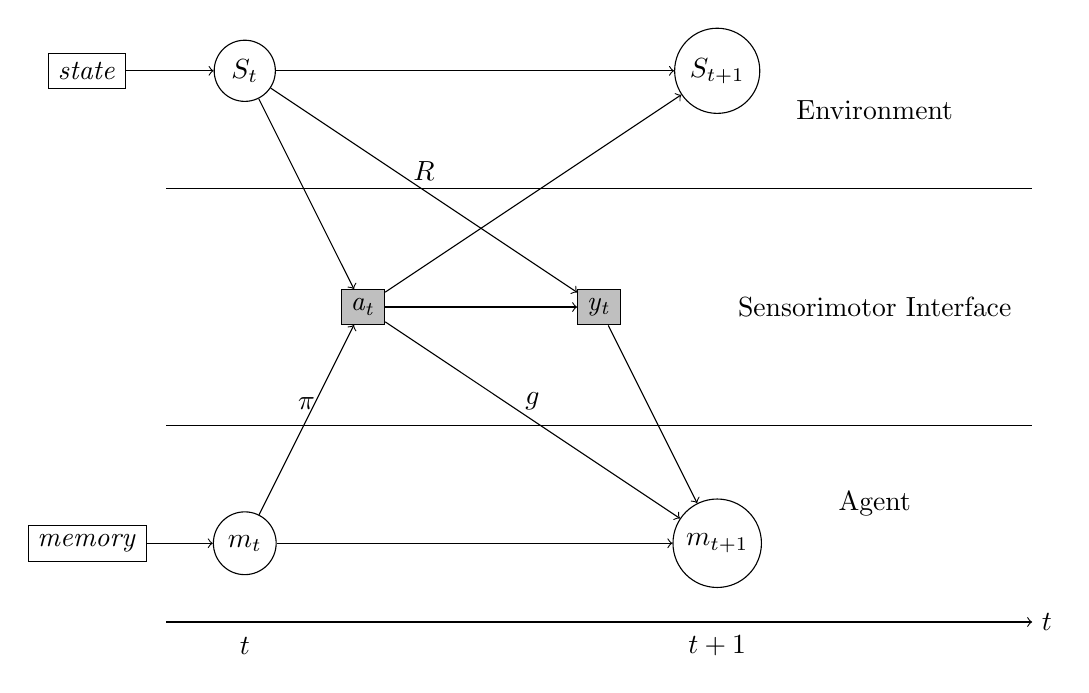
\begin{tikzpicture}

        % Time axis
        \draw[->] (-4, -4) -- (7, -4) node[right] {\(t\)};
        
        % Time labels
        \node at (-3, -4.3) {\(t\)};
        \node at (3, -4.3) {\(t+1\)};

        % Lines
        \draw (-4, -1.5) -- (7, -1.5) node[right] {};
        \draw (-4, 1.5) -- (7, 1.5) node[right] {};

        % Nodes
        \node (m_t) [circle, draw] at (-3, -3) {\(m_t\)};
        \node (a_t) [rectangle, draw, fill=gray!50] at (-1.5, 0) {\(\mathit{a_t}\)};
        \node (m_t1) [circle, draw] at (3, -3) {\(m_{t+1}\)};
        \node (y_t) [rectangle, draw, fill=gray!50] at (1.5,0) {\(\mathit{y_t}\)};
        \node (S_t) [circle, draw] at (-3, 3) {\(S_t\)};
        \node (S_t1) [circle, draw] at (3, 3) {\(S_{t+1}\)};

        \node (state) [rectangle, draw] at (-5, 3) {\(\mathit{state}\)};
        \node (memory) [rectangle, draw] at (-5, -3) {\(\mathit{memory}\)};
        
        % Edges
        \draw[->] (m_t) -- (m_t1);
        \draw[->] (m_t) -- (a_t) node[midway, above] {\(\pi\)};
        \draw[->] (a_t) -- (y_t);
        \draw[->] (a_t) -- (S_t1);
        \draw[->] (a_t) -- (m_t1) node[midway, above] {\(g\)};
        \draw[->] (S_t) -- (S_t1);
        \draw[->] (S_t) -- (a_t);
        \draw[->] (S_t) -- (y_t) node[midway, above] {\(R\)};
        \draw[->] (y_t) -- (m_t1);

        \draw[->] (state) -- (S_t);
        \draw[->] (memory) -- (m_t);

        % Additional text annotations
        \node at (5, 2.5) {Environment};
        \node at (5, -2.5) {Agent};
        \node at (5, 0) {Sensorimotor Interface};
        
    \end{tikzpicture}
\end{center}

\begin{itemize}
    \item $\pi(a|m) \to$ policy
    \item $R(y) \to $ reward function
    \item $p(s'y|sa) \to$ model of the environment
    \item $g(m'|may) \to$ memory update
\end{itemize}

The goal is to find the optimal policy $\pi^*$ that maximizes the expected return:

\[
maximize_{\pi} \underbrace{\mathbb{E} \left[ \sum_{t=0}^{\infty} \gamma^t R(y_t) \right]}_{Expected Return} \hspace{1cm} 0 \leq \gamma < 1
\]

with $\gamma$ survival probability.

The expected survival time is:
\[
    \frac{1}{1 - \gamma}
\]

Specifications:

\begin{itemize}
    \item \textbf{Perfect observability} $\to$ the agent knows the state of the environment ($y = S$) and $p(y|sas') = \mathcal{1}(y = s')$
    \begin{observationblock} 
        $$
        p(s'y|sa) = p(s'|sa)p(y|sas')
        $$
    \end{observationblock}
    \item \textbf{Memory update} $\to$ the agent knows the state of the environment and the memory ($M = y$) and $g(m'|may) = \mathcal{1}(m' = y)$
\end{itemize}

\section{Markov Decision Process}

\begin{definitionblock}[Markov Decision Process]
    A Markov Decision Process (MDP) is a fully observable set of tuples $(S, A, R, P, \gamma)$ where:
    \begin{itemize}
        \item $s \in S$ is a finite set of states
        \item $a \in A$ is a finite set of actions
        \item $R: S \times A \to \mathbb{R}$ is the reward function
        \item $P: S \times A \times S \to [0, 1]$ is the transition probability function
        \item $\gamma \in [0, 1]$ is the discount factor
        \item $p(s'y|sa)$ is the model of the environment
        \item $p_0(s)$ is the initial state distribution
        \item $\pi(a|s)$ is the policy
    \end{itemize}
\end{definitionblock}

\begin{figure}[H]
    \centering
    
\includegraphics[width=0.6\textwidth]{assets/fig1.png}
    \caption{Markov Decision Process}
    \label{fig:fig1}
\end{figure}

$$
\begin{array}{rl}
    G_{\pi}(\rho_0) 
    & = \mathbb{E} \left( \sum_{t=0}^{\infty} \gamma^t R(y_t) \right)\\
    & = \sum_{t=0}^{\infty} \gamma^t \mathbb{E} \left[ R(y_t) \right] \\
    & = \sum_{t=0}^{\infty} \gamma^t \sum_{sa}\rho_t(s)\pi(a|S)p(s'y|sa)r(y) \\
    & = \sum_{t=0}^{\infty} \gamma^t \sum_{s\in s'}\rho_t(s)\pi(a|s)p(s'|sa)r(sas') \\
\end{array}
$$

The difficulty here is that the dependence on $\pi$ is non linear, but linear on the initial condition. 

Let's introduce now the \textbf{Chapman Kolmogorov equation}:
$$
\rho_{t+1}(s') = \sum_{sa}\rho_t(s)\pi(a|s)p(s'|sa)
$$
it basically tells us that the probability of being in state $s'$ at time $t+1$ is the sum of the probabilities of being in state $s$ at time $t$ and then moving to state $s'$ by taking action $a$.

$$
\begin{array}{rl}
    G_{\pi}(\rho_0) 
    & = \sum_{s}\rho_0(s)\underbrace{V_{\pi}(s)}_{\text{value of the policy $\pi$}} \hspace{0.5cm} \rho_0 = e_s \text{ and } G_{\pi}(e_s) = V_{\pi}(s)\\
    & = \sum_{sas'}\rho_0(s)\pi(a|s)p(s'|sa)r(sas') + \gamma \underbrace{\sum_{t=1}^{\infty}\gamma^{t-1}\sum_{sas'}\rho_{t+1}(s)\pi(a|s)p(s'|sa)r(sas')}_{G_{\pi}(\rho_1)} \\
\end{array}
$$
The recursion equation is:
$$
V_{\pi}(s) = \sum_{a}\pi(a|s)\sum_{s'}p(s'|sa)[r(sas') + \gamma V_{\pi}(s')]
$$
one can also prove that it has a unique solution.
It is also the basis for evaluating the policy $\pi$.

The problem is that we want to find the optimal policy $\pi^*$ that maximizes the expected return seen before. 

$$
\pi^* = argmax_{\pi} G_{\pi}(\rho_0)
$$

For this purpose we introduce the \textbf{Bellman equation}:
$$
V^*(s) = \max_{a} \left[ r(s, a) + \gamma \sum_{s'} p(s'|s, a) V^*(s') \right]
$$

$$
\bar{\pi} = \mathds{1} (a = argmax_{a} \left[ \sum_{s'}p(s'sa)(r(sas') + \gamma V^*(s'))\right])
$$

\begin{enumerate}
    \item $V^*(s) = V_{\bar{\pi}}(s)$
    
    Recursion equation:
    $$
    \begin{array}{rl}
        V_{\bar{\pi}}(s) = \sum_{as'}\bar{\pi}(a|s)p(s'|sa)[r(sas') + \gamma V_{\bar{\pi}}(s')]\\
        V^*(s) = \sum_{as'}\bar{\pi}(a|s')p(s'|sa)[r(sas') + \gamma V^*(s')] \\
    \end{array}
    $$

    That leads to:
    $$
    (V_{\bar{\pi}}(s) - V^*(s)) = \sum_{a}\bar{\pi}(a|s)\sum_{s'}p(s'|sa)[r(sas') + \gamma V^*(s')] - \max_{a} \left[ r(s, a) + \gamma \sum_{s'} p(s'|s, a) V^*(s') \right]
    $$

    \item $G_{\bar{\pi}}(\rho_0) \geq G_{\pi}(\rho_0)$
    $$
    \begin{array}{rl}
        G_{\bar{\pi}}(\rho_0) 
        & = \sum_{s}\rho_0(s)V_{\bar{\pi}}(s)\\
        & = \sum_{s}\rho_0(s)V^*(s)\\
        & = \sum_{s}\rho_0(s) max_a \left[ \sum_{s'}p(s'|sa)[r(sas') + \gamma V^*(s')] \right] \\
        & \geq \sum_{sa}\rho_0(s)\pi(a|s) \sum_{s'}p(s'|sa)[r(sas') + \gamma V^*(s')] \\
        & = sum_{sas'}\rho_0(s)\pi(a|s)p(s'|sa)r(sas') + \underbrace{\gamma \sum_{sas'}\rho_0(s)\pi(a|s)p(s'|sa)V^*(s')}_{G_{\pi}(\rho_1)} \\

    \end{array}
    $$
\end{enumerate}

Let's intrduce the \textbf{Bellman Operator}:
$$
BW(s) = \max_{a} \left[ r(s, a) + \gamma \sum_{s'} p(s'|s, a) V(s') \right]
$$

The Bellman Operator is a contraction mapping:
$$
\begin{array}{rl}
    ||BW(s) - BW(s')|| 
    & = ||\max_{a} \left[ r(s, a) + \gamma \sum_{s'} p(s'|s, a) V(s') \right] - \max_{a} \left[ r(s', a) + \gamma \sum_{s'} p(s'|s', a) V(s') \right]|| \\
    & \leq ||r(s, a) - r(s', a)|| + \gamma ||\sum_{s'} p(s'|s, a) V(s') - \sum_{s'} p(s'|s', a) V(s')|| \\
    & \leq ||r(s, a) - r(s', a)|| + \gamma ||V(s) - V(s')|| \\
\end{array}
$$

$\gamma$ controls the contraction.








